\subsection{A learnable zero-start gate lowers worst-group accuracy}

With Qwen3.5-4B and SigLIP-base features, three connectors reach similar worst-group accuracy, and the gated
cross-attention connector with a learnable gate falls well below them (Table \ref{tab:main}, Figure \ref{fig:main}).

\begin{table*}[t]
\centering
\caption{Test worst-group accuracy (\%), mean ± s.d. over seeds (number of seeds in brackets), Qwen3.5-4B. With 5 seeds the MLP projector and Q-Former give 74.4 and 72.8 on Waterbirds and 66.2 and 69.2 on Watermark. \label{tab:main}}
\footnotesize
\begin{tabular}{@{}
  >{\raggedright\arraybackslash}p{(\linewidth - 8\tabcolsep) * \real{0.1667}}
  >{\centering\arraybackslash}p{(\linewidth - 8\tabcolsep) * \real{0.2083}}
  >{\centering\arraybackslash}p{(\linewidth - 8\tabcolsep) * \real{0.2083}}
  >{\centering\arraybackslash}p{(\linewidth - 8\tabcolsep) * \real{0.2083}}
  >{\centering\arraybackslash}p{(\linewidth - 8\tabcolsep) * \real{0.2083}}@{}}
\toprule
\begin{minipage}[b]{\linewidth}\raggedright
Task
\end{minipage} & \begin{minipage}[b]{\linewidth}\centering
MLP projector
\end{minipage} & \begin{minipage}[b]{\linewidth}\centering
Q-Former
\end{minipage} & \begin{minipage}[b]{\linewidth}\centering
Learnable gate
\end{minipage} & \begin{minipage}[b]{\linewidth}\centering
Fixed gate
\end{minipage} \\
\midrule
Waterbirds & 74.5 ± 1.5 (3) & 71.7 ± 2.5 (3) & 63.6 ± 10.4 (15) & 74.2 ± 3.4 (15) \\
Watermark & 63.6 ± 4.4 (3) & 68.6 ± 4.1 (3) & 40.5 ± 18.0 (15) & 65.7 ± 10.3 (15) \\
\bottomrule
\end{tabular}
\end{table*}

\begin{figure*}[t]
\centering
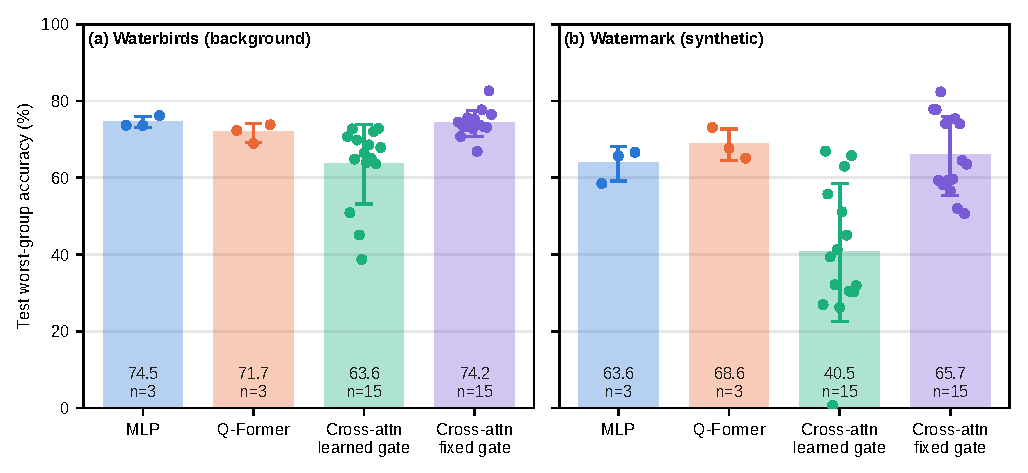
\includegraphics[width=\linewidth]{figures/main_connectors.pdf}
\caption{Test worst-group accuracy of the four connectors (Qwen3.5-4B, SigLIP-base) on (a) Waterbirds and (b) Watermark. Bars are means with one standard deviation; dots are single seeds; hatching distinguishes connectors; the numbers under each bar give the mean and the number of seeds. Only the learnable, zero-start gate fails, and it is also the least stable}\label{fig:main}
\end{figure*}

Fixing the gate raises worst-group accuracy in all four LLM and task cells (Table \ref{tab:h1}, Figure \ref{fig:forest}). The
effects are large (\(d_z\) = 1.10 and 1.34 on Qwen3.5-4B) and every cell survives Holm correction (largest adjusted
\(p\) = 0.009). The result holds when the checkpoint is chosen without group labels (+17.7 and +25.5 points), with
unpaired Welch and Mann--Whitney tests (all \(p \le 0.002\)), and on the confirmation seeds alone (Waterbirds +10.5,
\(p = 9.5 \times 10^{-4}\); Watermark +26.7, \(p = 2.5 \times 10^{-4}\)). The fixed gate also raises average accuracy
(84.1 to 88.0 on Waterbirds, 76.9 to 86.1 on Watermark), so the gain is not a trade against average accuracy.

\begin{table*}[t]
\centering
\caption{Hypothesis H1, paired by seed. One-sided paired t-test at \(\alpha = 0.025\); all four cells survive Holm
correction. Collapsed runs have worst-group accuracy below 50\%. On Phi-4-mini Watermark, seeds 5 to 9 were added
after the 5-seed test missed \(\alpha\) (\(p = 0.044\)); tested alone they give \(p = 0.023\). \label{tab:h1}}
\footnotesize
\begin{tabular}{@{}
  >{\raggedright\arraybackslash}p{(\linewidth - 14\tabcolsep) * \real{0.1053}}
  >{\raggedright\arraybackslash}p{(\linewidth - 14\tabcolsep) * \real{0.1053}}
  >{\centering\arraybackslash}p{(\linewidth - 14\tabcolsep) * \real{0.1316}}
  >{\centering\arraybackslash}p{(\linewidth - 14\tabcolsep) * \real{0.1316}}
  >{\centering\arraybackslash}p{(\linewidth - 14\tabcolsep) * \real{0.1316}}
  >{\centering\arraybackslash}p{(\linewidth - 14\tabcolsep) * \real{0.1316}}
  >{\centering\arraybackslash}p{(\linewidth - 14\tabcolsep) * \real{0.1316}}
  >{\centering\arraybackslash}p{(\linewidth - 14\tabcolsep) * \real{0.1316}}@{}}
\toprule
\begin{minipage}[b]{\linewidth}\raggedright
LLM
\end{minipage} & \begin{minipage}[b]{\linewidth}\raggedright
Task
\end{minipage} & \begin{minipage}[b]{\linewidth}\centering
Seeds
\end{minipage} & \begin{minipage}[b]{\linewidth}\centering
Learnable
\end{minipage} & \begin{minipage}[b]{\linewidth}\centering
Fixed
\end{minipage} & \begin{minipage}[b]{\linewidth}\centering
Gain {[}95\% CI{]}
\end{minipage} & \begin{minipage}[b]{\linewidth}\centering
H1 \(p\)
\end{minipage} & \begin{minipage}[b]{\linewidth}\centering
Collapsed (learnable / fixed)
\end{minipage} \\
\midrule
Qwen3.5-4B & Waterbirds & 15 & 63.6 & 74.2 & +10.6 {[}5.3, 16.0{]} & \(4 \times 10^{-4}\) & 2 / 0 \\
Qwen3.5-4B & Watermark & 15 & 40.5 & 65.7 & +25.2 {[}14.8, 35.6{]} & \(7 \times 10^{-5}\) & 10 / 0 \\
Phi-4-mini & Waterbirds & 5 & 60.4 & 70.1 & +9.7 {[}3.8, 15.7{]} & 0.005 & 0 / 0 \\
Phi-4-mini & Watermark & 10 & 29.4 & 54.9 & +25.5 {[}8.2, 42.7{]} & 0.004 & 8 / 6 \\
\bottomrule
\end{tabular}
\end{table*}

\begin{figure}[t]
\centering
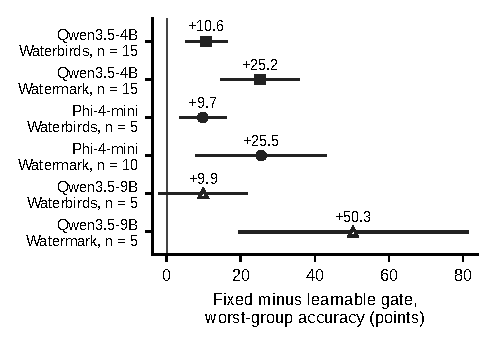
\includegraphics[width=\linewidth]{figures/forest_gain.pdf}
\caption{Paired gain from fixing the gate (fixed minus learnable gate, worst-group accuracy points) with 95\% confidence intervals; squares Qwen3.5-4B, circles Phi-4-mini}\label{fig:forest}
\end{figure}

The learnable gate also makes robustness depend on the seed (H2). On Qwen3.5-4B its variance is higher on both tasks
(variance-ratio \(p = 9 \times 10^{-5}\) and 0.02) and it collapses in 2 of 15 and 10 of 15 runs, against none for
the fixed gate (Figure \ref{fig:seeds}). On Phi-4-mini the variance difference is not significant (\(p\) = 0.20 and
0.23), and on Watermark the fixed gate still collapses in 6 of 10 runs.

\begin{figure*}[t]
\centering
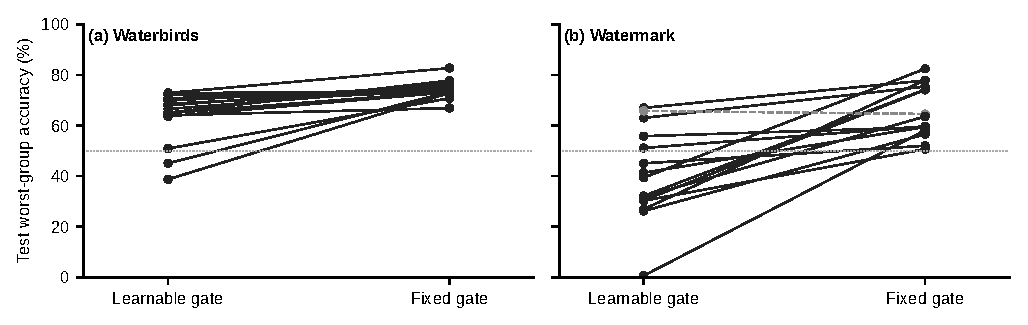
\includegraphics[width=\linewidth]{figures/h1_seeds_qwen.pdf}
\caption{Each line joins one paired run of the learnable gate to the fixed gate (Qwen3.5-4B) on (a) Waterbirds and (b) Watermark. Solid lines rise and dashed lines fall; the dotted line marks the 50\% collapse threshold}\label{fig:seeds}
\end{figure*}

\subsection{The zero start, not learnability, is the cause}

Controls change one property of the learnable gate at a time (Table \ref{tab:controls}; all exploratory).

\begin{table*}[t]
\centering
\caption{Controls on Qwen3.5-4B, test worst-group accuracy (\%), Waterbirds / Watermark unless stated. \label{tab:controls}}
\footnotesize
\begin{tabular}{@{}
  >{\raggedright\arraybackslash}p{(\linewidth - 8\tabcolsep) * \real{0.1739}}
  >{\centering\arraybackslash}p{(\linewidth - 8\tabcolsep) * \real{0.2174}}
  >{\centering\arraybackslash}p{(\linewidth - 8\tabcolsep) * \real{0.2174}}
  >{\centering\arraybackslash}p{(\linewidth - 8\tabcolsep) * \real{0.2174}}
  >{\raggedright\arraybackslash}p{(\linewidth - 8\tabcolsep) * \real{0.1739}}@{}}
\toprule
\begin{minipage}[b]{\linewidth}\raggedright
Control
\end{minipage} & \begin{minipage}[b]{\linewidth}\centering
Seeds
\end{minipage} & \begin{minipage}[b]{\linewidth}\centering
Learnable variant
\end{minipage} & \begin{minipage}[b]{\linewidth}\centering
Reference
\end{minipage} & \begin{minipage}[b]{\linewidth}\raggedright
What it shows
\end{minipage} \\
\midrule
Learnable gate started open (\(\tanh\alpha_0 = 0.995\)) & 5 & 71.8 / 66.8 & fixed 72.9 / 72.1 & starting open removes most of the gap \\
Fixed gate with injection capped at the text norm & 5 & 69.9 / 50.6 & zero start 61.2 / 42.6; fixed 73.1 / 67.2 & keeps part of the gain on Waterbirds (\(-3.2\) against fixed, \(p\) = 0.13) but loses most on Watermark (\(-16.6\), \(p\) = 0.002); 2 of 5 Watermark seeds collapse \\
Learnable gate started at \(\tanh\alpha_0 = 0.01\) & 5 & 69.1 / 22.5 & zero start 61.2 / 42.6; fixed 73.1 / 67.2 & gate falls back to 0.001 to 0.008; Watermark collapses in 5 of 5 seeds, \(-20.1\) below the zero start (\(p\) = 0.041) \\
Learnable gate started at \(\tanh\alpha_0 = 0.1\) & 5 & 73.1 / 65.3 & zero start 61.2 / 42.6; fixed 73.1 / 67.2 & +11.9 and +22.7 over the zero start (\(p\) = 0.041, 0.072); no difference from the fixed gate \\
Learnable gate started half open (\(\tanh\alpha_0 = 0.5\)) & 5 & 72.6 / 62.7 & zero start 61.2 / 42.6; fixed 73.1 / 67.2 & +11.4 and +20.1 over the zero start (\(p\) = 0.014, 0.006); no difference from the fixed gate \\
Gate excluded from gradient clipping & 3 & 67.2 / 52.9 & zero start, same seeds 64.4 / 39.3 & no significant change; gate stays below 0.003 \\
No weight decay on the gate & 2 & 52.2 / 28.0 & zero start, same seeds 60.9 / 44.9 & no rescue \\
Connector learning rate \(5 \times 10^{-5}\) / \(2 \times 10^{-4}\) / \(10^{-3}\) (Waterbirds) & 2 & 35.9 / 56.8 / 65.8 & fixed 65.6 / 73.5 / 66.5 & the gap shrinks as the gate moves further (final 0.002 / 0.004 / 0.018) \\
fp16 weights instead of 4-bit & 3 & 63.2 / 44.1 & fixed 73.2 / 65.1 & same direction (+10.0, +21.1; not significant with 3 seeds) \\
Eight training epochs (Waterbirds) & 4 & 67.9 & fixed 79.0 & +11.0 (\(p\) = 0.023); one of five fixed-gate runs collapsed \\
\bottomrule
\end{tabular}
\end{table*}

A learnable gate that starts half open behaves like the fixed gate and moves little (final \(\tanh\alpha\) 0.44),
so the outcome depends on where the gate starts rather than on whether it can learn. A start of 0.1 is already
enough. That gate shrinks during training, to 0.058 to 0.064, but stays about a hundred times above the zero-start
gate, and its worst-group accuracy equals the fixed gate's on Waterbirds (73.1 against 73.1). Its gradient also
changes sign often: 27\% to 51\% of steps per epoch push the gate up, with a slight net push down. A start of 0.01
is not enough. That gate falls back to the zero-start range (final \(|\tanh\alpha|\) 0.001 to 0.008), and Watermark
collapses below 50\% in all five seeds (22.5, against 42.6 for the zero start). Because this control also starts
\(W_o\) at zero, the gradient of \(W_o\) is scaled by the small gate, which may explain why it ends below the zero
start. The threshold therefore lies between 0.01 and 0.1. Ten times longer alignment
leaves the zero-start gate below 0.003 but also destabilises the learnable-gate alignment (caption loss rises from
2.0 to 7.9), so that run shows fragility rather than a clean effect and is reported only in the supplement.

\subsection{The gate's gradient is large but cancels itself}

After alignment the zero-start gate sits at \(|\tanh\alpha| \approx 0.0005\) and never exceeds 0.01. Its gradient is
not small: the mean absolute pre-clipping gradient per epoch ranges from 3 to 1,528 across 13 learnable-gate runs,
and in some runs it is almost all of the global gradient norm. With Adam, each step moves \(\alpha\) by at most about
the learning rate \(\eta = 2 \times 10^{-4}\), so over the roughly 900 to 1,200 task steps a gradient of constant sign
would move \(\alpha\) by up to about 0.2. The observed change is below 0.003. The gradient must therefore change sign
from step to step and cancel. The signed gradient, logged in seven further zero-start runs, confirms this: the mean
absolute gradient reaches 37 to 1,282 per epoch, yet 37\% to 60\% of steps push the gate up, the sign changes on 45\%
to 49\% of consecutive steps, and the gate ends at 0.001 to 0.005. The gate started at 0.01 behaves the same way
(30\% to 58\% of steps push it up). This differs from the dead-gradient account of \citep{farazi2026gate}, which requires an
injected signal that does not depend on the text; ours does.

\subsection{The pathway is weak, not closed}

The learnable gate passes 15 to 35 times less visual signal than the fixed gate (injection ratio 3.5 against 112,
6 runs each), because \(W_o\) grows to partly offset the small gate. Removing the visual pathway at inference, or
zeroing the image features, makes the learnable-gate model give the same answer to every image in every run:
average accuracy falls from 83.0 to the share of one class on Waterbirds (\(-46.9\) points, 4 of 4 seeds, \(p\) = 0.035)
and from 81.8 to 50.0 on Watermark (3 of 3 seeds, \(p\) = 0.003). The fixed-gate model does the same. The learnable
gate therefore still uses the image; its pathway is weak, not closed. In these runs the fixed gate again led on
worst-group accuracy (+16.2 on Waterbirds, 4 seeds; +14.4 on Watermark, 3 seeds). Within learnable-gate runs the injection ratio does not predict
worst-group accuracy (Spearman \(\rho\) = 0.33, \(p\) = 0.27). Both gate variants attend to the watermark corner more
than to the rest of the image (16.7\% and 18.2\% of attention against 8.2\% if uniform), yet only the learnable-gate
model relies on it.

\subsection{Connector type matters little once the gate is fixed}

MLP projector and Q-Former do not differ significantly (5 seeds; \(p\) = 0.23 on Waterbirds and 0.40 on Watermark),
and neither differs significantly from the fixed gate, although equivalence within three points is not established.
Matching the number of image tokens (36 instead of 49 MLP tokens) changes nothing (74.7 against 74.9). The fixed-gate
connector needs about half the step time and memory of the MLP projector (1.7 against 4.0 s per step; 6.2 against
12.1 GB on one T4).

\subsection{Boundaries of the effect}

\emph{Injection depth.} With four gated blocks inside the decoder, the learnable and fixed gates do not differ (Waterbirds
70.8 against 70.4, 5 seeds; Watermark 68.3 against 70.6, 4 seeds), although the per-layer learnable gates also stay
small (mean \(|\tanh\alpha|\) 0.027).

\emph{Encoder size.} With SigLIP-large every connector improves on Waterbirds by 6 to 11 points, and the gap narrows to
+8.0 (\(p\) = 0.09, 4 paired seeds). On Watermark it remains: 53.2 against 75.6 (+22.4, \(d_z\) = 0.85, \(p\) = 0.13,
5 seeds) (Figure \ref{fig:encoder}).

\emph{Third task.} On CelebA the direction is the same but not significant (43.5 against 51.1, +7.7, \(p\) = 0.48, 5 paired
seeds).

\emph{Shortcut strength.} At a 90\% watermark correlation all arms learn the task (learnable 75.7, fixed 77.5); at 99\% all
arms fail (6.7 and 20.1). The gap is largest at the 95\% used in the main experiment.

\emph{Group labels.} Group distributionally robust optimisation (Group DRO) \citep{sagawa2020groupdro}, which uses group labels in training, closes the gap on Waterbirds (+2.3, \(p\) = 0.70,
4 seeds) but not on Watermark (+17.5, \(p\) = 0.059).

\begin{figure*}[t]
\centering
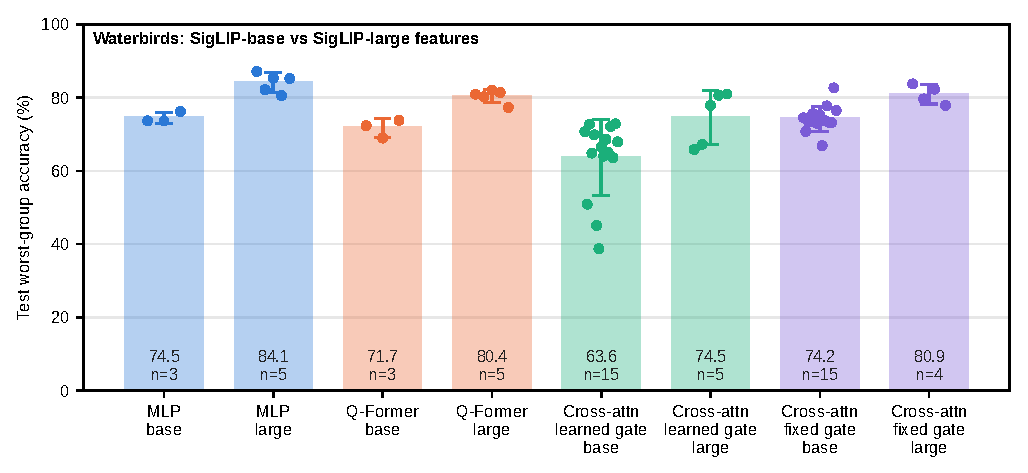
\includegraphics[width=\linewidth]{figures/encoder_scale.pdf}
\caption{Waterbirds worst-group accuracy with SigLIP-base and SigLIP-large features. Bars are means with one standard deviation, dots are single seeds, and the numbers under each bar give the mean and the number of seeds. Every connector gains from the larger encoder; the learnable gate still lags}\label{fig:encoder}
\end{figure*}

\subsection{Free-form answers under shifted priors}

On VQA-CP v2 every model loses 15 to 21 points when the answer priors shift, so the subset exposes the language
prior (Table \ref{tab:vqacp}). A text-only model with the same LLM, LoRA and budget sets the reference. The learnable gate does no
better than this model in distribution (47.6 against 48.2, \(p\) = 0.23), and removing its visual pathway changes
nothing, so it does not use the image at test time (injection ratio 0.05). Its 2.1-point lead under shifted priors
(\(p\) = 0.041) remains with the image removed (29.2), so it comes from training with the pathway present rather
than from the test image. The fixed gate is worse than having no image at all: \(-5.7\) points in distribution
against the text-only model (\(p\) = 0.001). Its injected signal is about 70 times the text norm, and removing it
raises shifted-prior accuracy by 4.6 points.

Capping the injected signal at the text norm removes this cost. The capped connector scores 49.6 in distribution and
30.6 under shifted priors, 7.0 points above the uncapped fixed gate in distribution (\(p\) = 0.020) and 3.5 points
above the text-only model under shifted priors (\(p\) = 0.028). It is also the only model whose accuracy depends on
the test image: removing the pathway or zeroing the image features costs 2.8
to 3.5 points in distribution and 1.0 to 2.0 under shifted priors (\(p\) = 0.041 to 0.063, 3 seeds). Strong injection
therefore disturbs free-form generation, and an injection held at the text norm avoids that while still using the
image. On the binary shortcut tasks, however, the cap gives back much of the fixed gate's gain (Table \ref{tab:controls}): Waterbirds
69.9 against 73.1 for the uncapped fixed gate (\(p\) = 0.13) and Watermark 50.6 against 67.2 (\(p\) = 0.002, \(d_z\) =
\(-3.1\)), with two of five Watermark seeds collapsed. The capped model still uses the image on these tasks: removing
the pathway makes it give one answer to every image. Injection strength therefore trades shortcut robustness on a
class readout against the quality of free-form answers.

\begin{table*}[t]
\centering
\caption{VQA-CP v2 subset, VQA accuracy (\%), mean ± standard deviation over 3 seeds. Prior answer rate: share of answers
equal to the most frequent training answer for the question type (same priors / shifted priors). Not comparable with
published VQA-CP results. \label{tab:vqacp}}
\footnotesize
\begin{tabular}{@{}
  >{\raggedright\arraybackslash}p{(\linewidth - 12\tabcolsep) * \real{0.1176}}
  >{\centering\arraybackslash}p{(\linewidth - 12\tabcolsep) * \real{0.1471}}
  >{\centering\arraybackslash}p{(\linewidth - 12\tabcolsep) * \real{0.1471}}
  >{\centering\arraybackslash}p{(\linewidth - 12\tabcolsep) * \real{0.1471}}
  >{\centering\arraybackslash}p{(\linewidth - 12\tabcolsep) * \real{0.1471}}
  >{\centering\arraybackslash}p{(\linewidth - 12\tabcolsep) * \real{0.1471}}
  >{\centering\arraybackslash}p{(\linewidth - 12\tabcolsep) * \real{0.1471}}@{}}
\toprule
\begin{minipage}[b]{\linewidth}\raggedright
Model
\end{minipage} & \begin{minipage}[b]{\linewidth}\centering
Test, same priors
\end{minipage} & \begin{minipage}[b]{\linewidth}\centering
Image removed
\end{minipage} & \begin{minipage}[b]{\linewidth}\centering
Test, shifted priors
\end{minipage} & \begin{minipage}[b]{\linewidth}\centering
Image removed
\end{minipage} & \begin{minipage}[b]{\linewidth}\centering
Prior answer rate
\end{minipage} & \begin{minipage}[b]{\linewidth}\centering
Injection ratio
\end{minipage} \\
\midrule
Text only & 48.2 ± 0.4 & n/a & 27.1 ± 0.1 & n/a & 39.9\% / 35.0\% & 0 \\
Learnable gate & 47.6 ± 0.2 & 47.6 ± 0.2 & 29.1 ± 0.8 & 29.2 ± 0.7 & 39.9\% / 33.2\% & 0.05 \\
Fixed gate & 42.6 ± 0.7 & 40.4 ± 0.9 & 27.6 ± 0.8 & 32.2 ± 0.4 & 33.8\% / 31.1\% & 70.1 \\
Capped injection & 49.6 ± 1.7 & 46.7 ± 0.4 & 30.6 ± 0.9 & 29.7 ± 1.2 & 39.0\% / 32.7\% & 1.00 \\
\bottomrule
\end{tabular}
\end{table*}

\subsection{A connector-only fix}

Retraining only the connector on half of the group-balanced validation set, with the LLM and LoRA frozen, lifts the
fixed-gate connector on Watermark from 72.5 to 89.6 ± 0.5 (5 seeds). This beats the same fix on the MLP projector
(81.2; +8.4, \(p < 0.001\)) and a linear probe trained the same way on the frozen features (85.1). On Waterbirds it
gives no gain (73.9 to 74.1) (Figure \ref{fig:fixes}). Qwen3.5-4B with its own vision tower, zero-shot and with a
threshold calibrated on validation, reaches only 35.5 on Waterbirds.

\begin{figure*}[t]
\centering
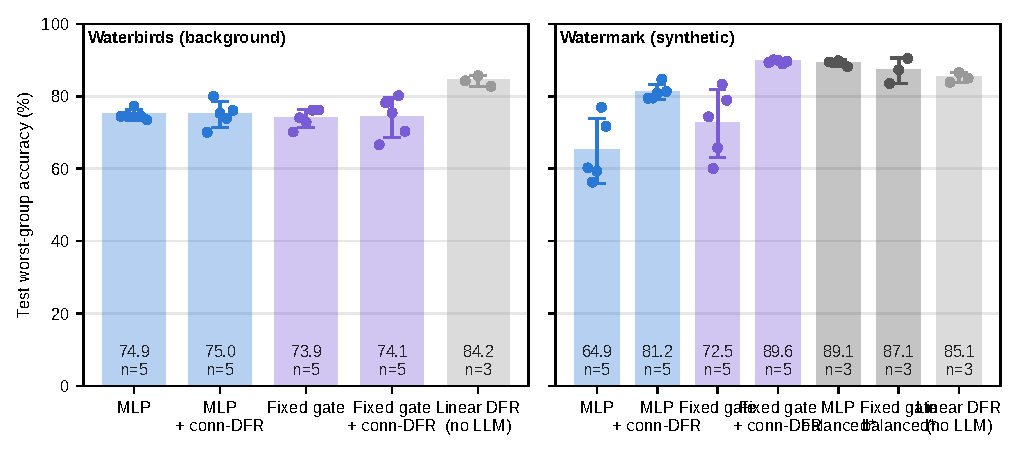
\includegraphics[width=\linewidth]{figures/fixes.pdf}
\caption{Connector-only deep feature reweighting (conn-DFR), group-balanced sampling and a linear probe on the frozen features. Bars are means with one standard deviation, dots are single seeds, and the numbers under each bar give the mean and the number of seeds; (a) Waterbirds, (b) Watermark. Starred bars use group labels during training (group-balanced sampling). Conn-DFR on the fixed gate reaches 89.6\% worst-group accuracy on Watermark and gives no gain on Waterbirds}\label{fig:fixes}
\end{figure*}

\subsection{Gates in released models}

The released weights of models that use the same zero-start tanh gates show the same regime. Nine of the 20
cross-attention gates of IDEFICS-80B have \(|\tanh\alpha| < 0.05\), and so do all gates of Llama 3.2 11B Vision (8 of 8)
and 90B Vision Instruct (20 of 20), whose values are at most 0.012. A small gate does not show that these models
ignore the image; we did not test them for shortcut reliance.
